\chapter{Results}



\section{Order Verification Study}
\label{sec:ord_ver_std}

	\subsection{Spacial Discretization}
	\label{sec:s_disc}
A grid refinement study was performed to verify the order of accuracy of the spatial discretizations discussed in Section \ref{sec:num_disc}.  In order to determine the error of the approximations, The Method of Manufactured Solutions was implemented.  A manufactured solution was selected, $\psi_{manu}$, and the analytic right hand side of the corresponding numerical scheme was computed.  The analytic right hand side was used in the numerical scheme, to compute a numerical solution, $\psi_{num}$, that satisfied the numerical scheme to a specified tolerance.  A tolerance of $10^{-12}$ was selected to ensure that the error owing from this tolerance would be negligible in comparison to the discretization error.  The total error could then be computed from Equation \ref{eq:tot_error}.


\begin{equation}
\label{eq:tot_error}
\epsilon = |(\psi_{manu} - \psi_{num})|
\end{equation}


Using Equation \ref{eq:tot_error}, the error for each point in a specific size grid was computed to determine the maximum error, $\epsilon_{max}$.  The maximum error was compared for different grid sizes, and the results are plotted on a log scale in Figure \ref{fig:ovs_sd}.  The dashed vertical lines indicate the minimum and maximum grid spacing that the numerical schemes will be implemented on.

\begin{figure}[h!]
\center
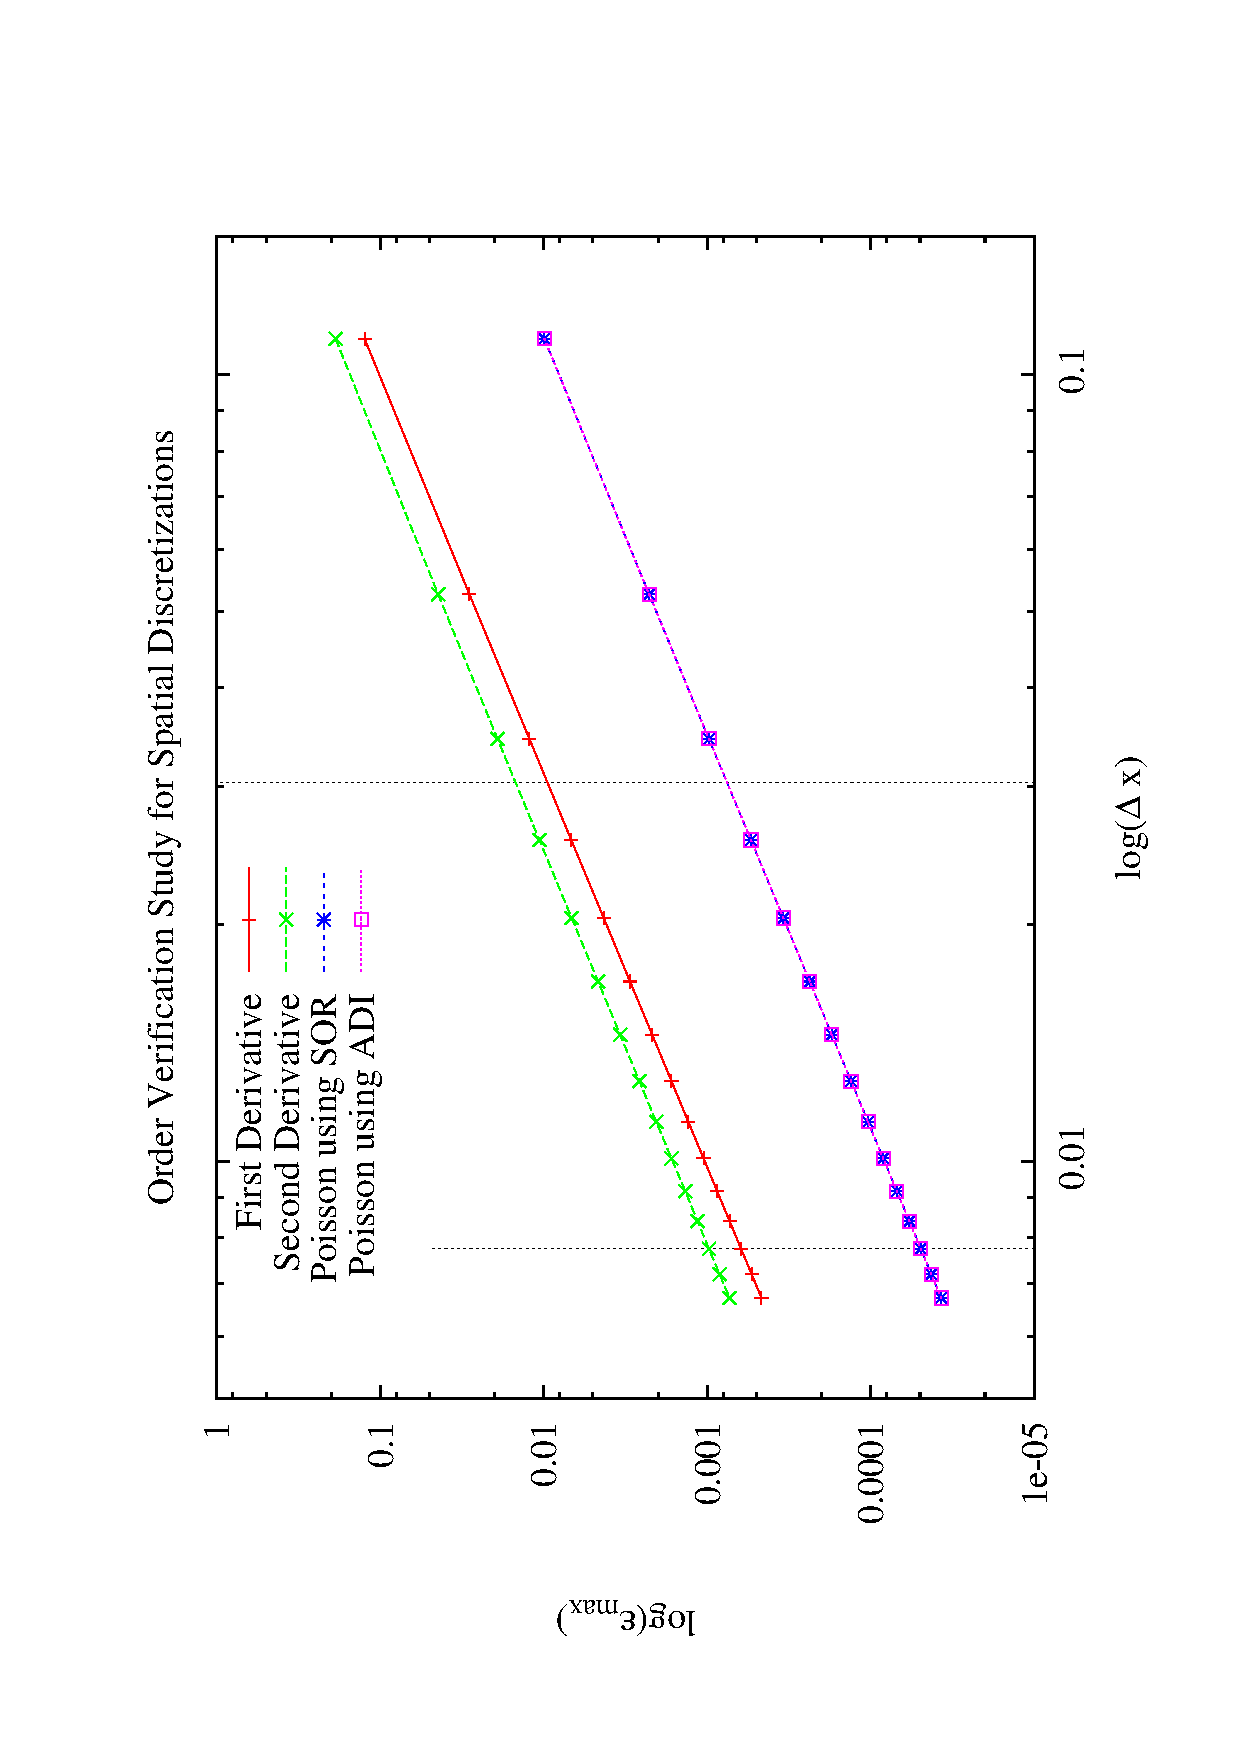
\includegraphics[width=0.9\textwidth]{plots/ovs_sd}
\caption{Maximum numerical error as a function of grid spacing for spatial discretizations, plotted on a log-log scale.}
\label{fig:ovs_sd}
\end{figure}

Using the plots in Figure \ref{fig:ovs_sd}, a linear curve was fit to the data, and the result are summarized in Table \ref{tab:ovs_sd}.  The slope of all the curves is approximately 2, therefore the maximum error in the grid is proportional to the square of the grid spacing, as shown in Proposition \ref{prop:log_slope}, and is consistent with the numerical schemes selected.  It can also be stated that for the selected grid sizes of interest for this study, the numerical error is mainly dominated by discretization error.


\begin{table}
\center
\caption{Summary of Slope Data for Figure \ref{fig:ovs_sd}}
\label{tab:ovs_sd}

\begin{tabular}{l c r}
\hline
Numerical Disc. & Slope & Error \\
\hline 
\hline 
$1^{st}$ Derivative & 1.99461 & $\pm$ 0.001142 \\
$1^{st}$ Derivative & 1.98334 & $\pm$ 0.003548 \\
Poisson w/ SOR      & 1.99383 & $\pm$ 0.001311 \\
Poisson w/ ADI      & 1.99384 & $\pm$ 0.001312 \\
\hline  
\end{tabular}
\end{table}



\begin{proposition}
\label{prop:log_slope}
  The slope of the log plot gives the power of the relationship between the two plotted variables.
\end{proposition}

\begin{proof}
  \begin{displaymath}
    \log(y) = a \log(x) + b \\ \\
    e^{\log(y)} = e^{a \log(x) + b } \\ \\
    y = c x^a \\ \\
    y  \propto  x^a \\     
  \end{displaymath}

\end{proof}

	\subsection{Temporal Discretization}
	\label{sec:t_disc}

A first order accurate temporal discretization was selected for these simulations because only steady state data was required, and the temporal discretization should have no effect on these results.  An order verification study wasn't performed on the temporal discretization, but instead two more simulations were run using two different time steps, to ensure that the steady state results were indifferent to changes in time step.  Unfortunately, some of the numerical precision was lost when the data was written out to file with only 7 decimal places of precision. The only conclusion that can be drawn is that the results were indifferent to 7 decimal places of precision.  

%NO INFO ADDED WITH THESE PLOTS. OMIT
%The data from this study is plotted in Figure \ref{fig:cfl_u} and \ref{fig:cfl_v}.
%
%\begin{figure}[h!]
%\label{fig:cfl_u}
%\center
%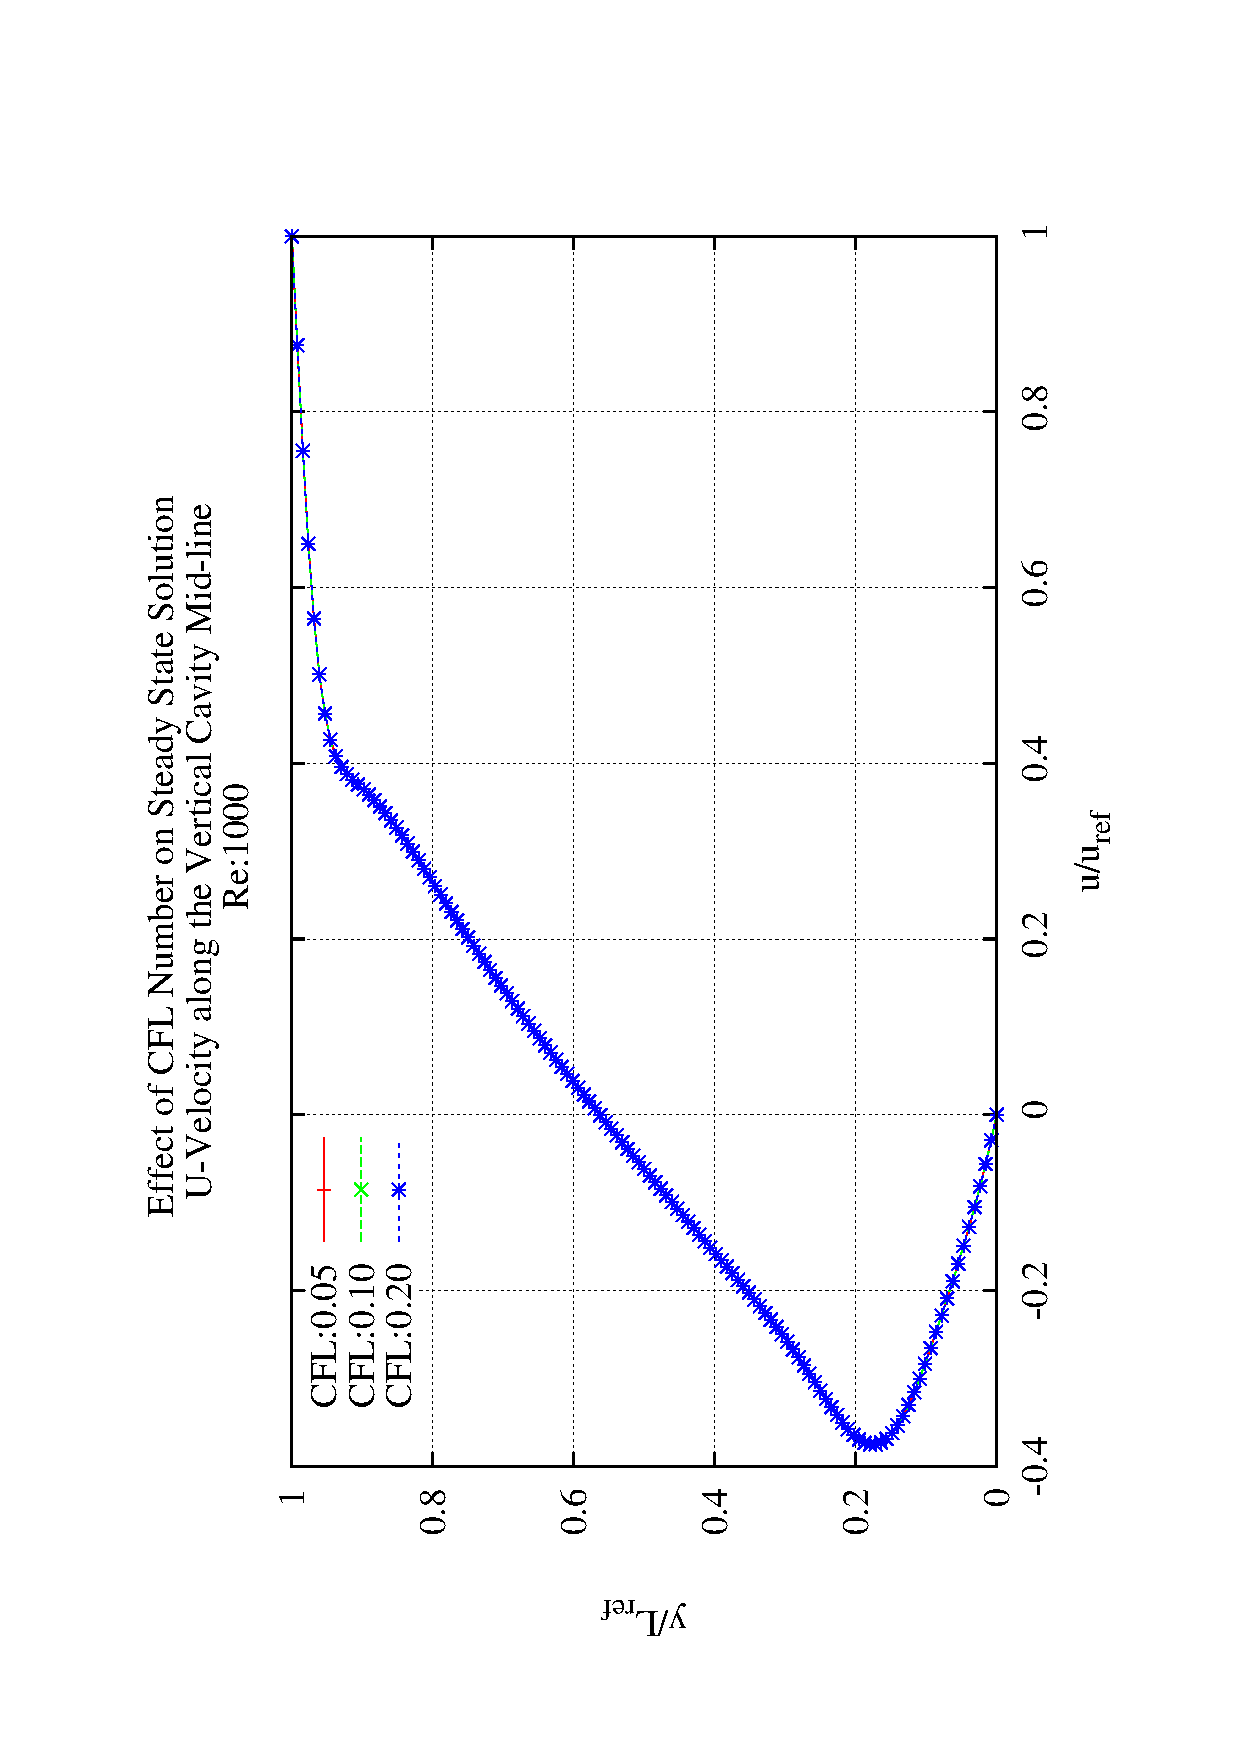
\includegraphics[width=0.9\textwidth]{plots/cfl_u}
%\caption{Steady state u-velocity as a function of y, along the vertical cavity mid-line, for 3 different CFL numbers, at Re:1000.}
%\end{figure}
%
%\begin{figure}[h!]
%\label{fig:cfl_v}
%\center
%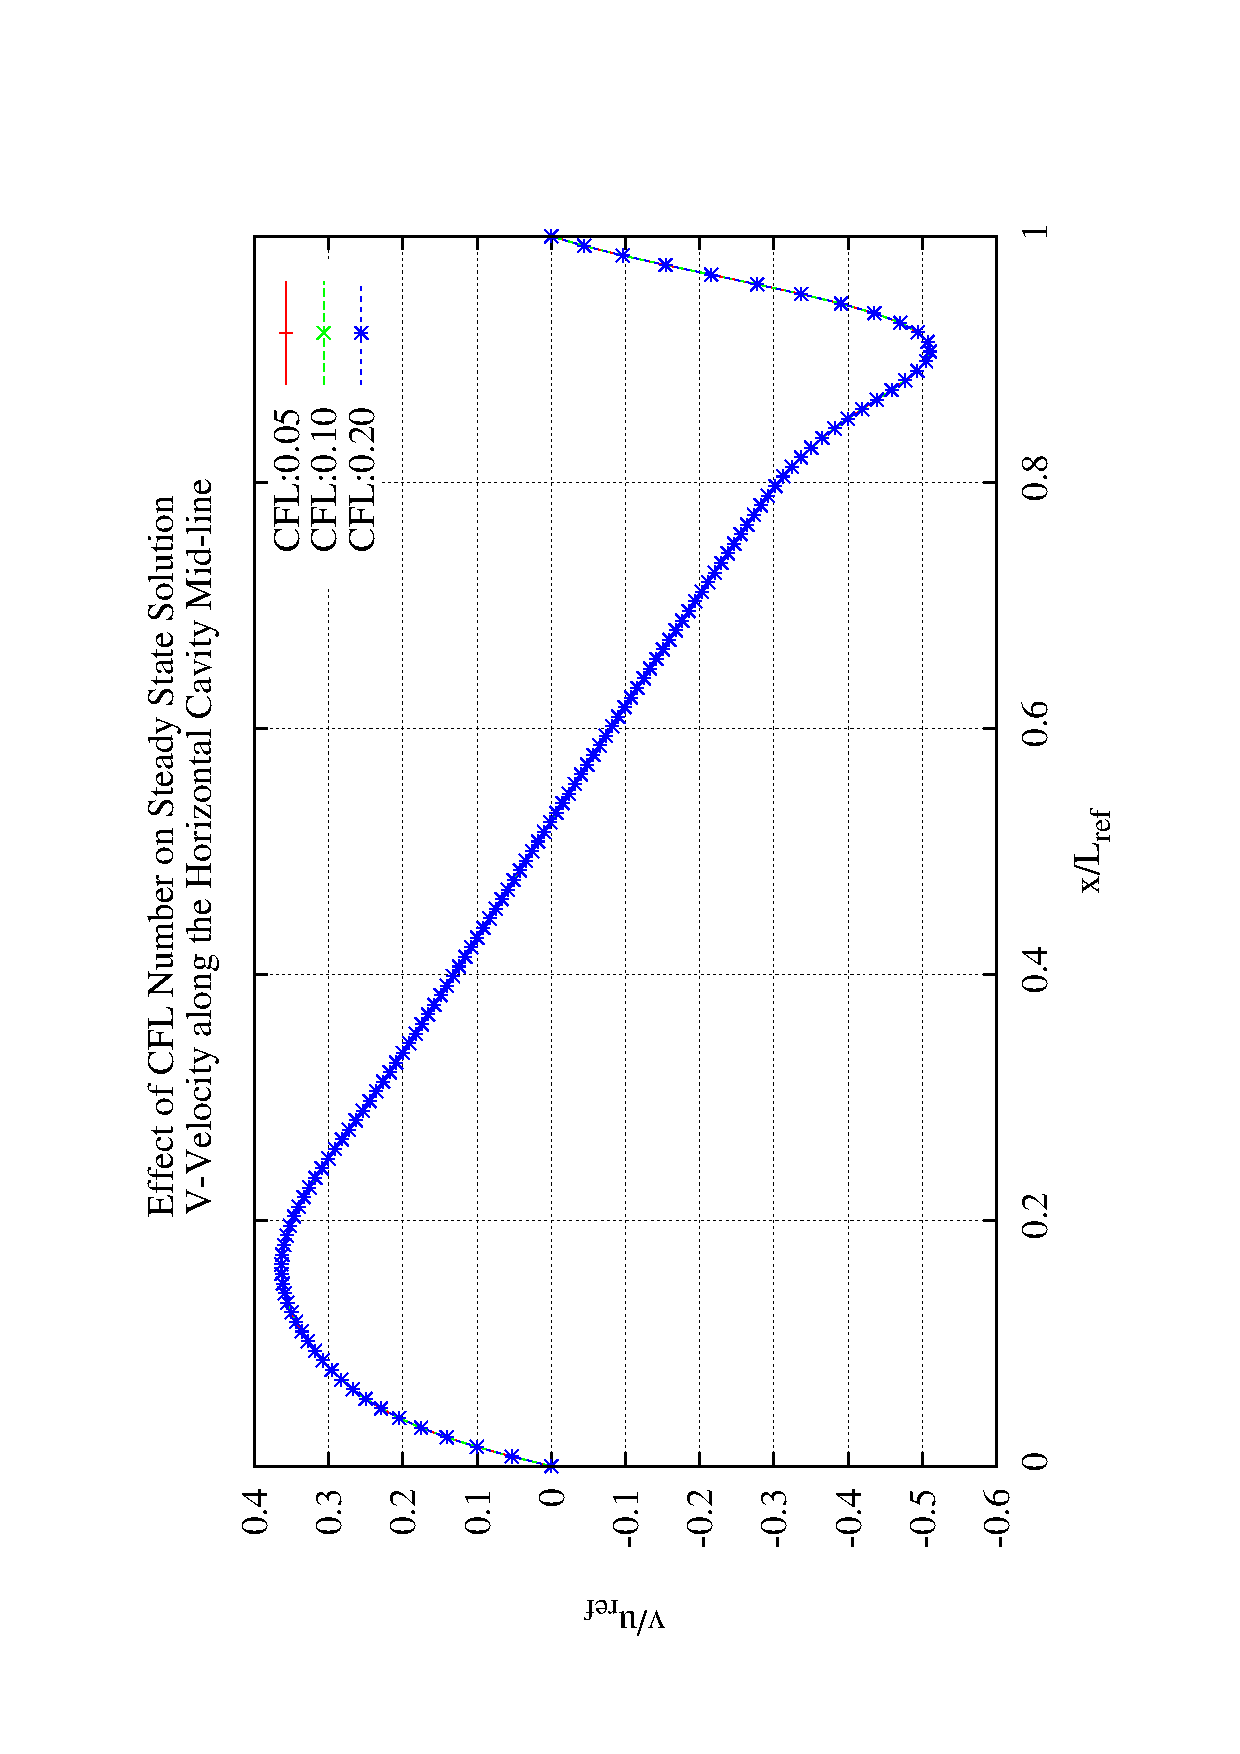
\includegraphics[width=0.9\textwidth]{plots/cfl_v}
%\caption{Steady state v-velocity as a function of x, along the horizontal cavity mid-line, for 3 different CFL numbers, at Re:1000.}
%\end{figure}
%
Additionally, instabilities were observed for a CFL number of 0.5, and the solution failed to converge. A stability analysis was not performed for the forward time, central space (FTCS) scheme implemented, so no comments can be made on this result.  The largest CFL number selected, that leads to stable solutions is 0.2.  There is very little resolution on where the stability limit is; the stability limit is somewhere between $0.2 < CFL < 0.5$.

%A video of the observed instabilities is available in Appendix /ref{app:instability}. 

\section{Optimizing Solution Algorithm}
\label{sec:opt_sol_alg}


	\subsection{Selection of Residual Tolerance}
	\label{sec:res_tol}

The residual tolerance was selected to be as large as possible, without compromising the accuracy of the numerical schemes selected.  This was done by varying the tolerance, performing an order verification study, as described in Section \ref{sec:ord_ver_std}, and observing the effect of tolerance on the solutions order of accuracy.  This process is shown, for both the SOR and ADI solvers, in Figures \ref{fig:rts} and \ref{fig:rta}.  The vertical lines correspond to the fine, medium and coarse grid respectively.

\begin{figure}[h!]
\center
\includegraphics[width=0.9\textwidth]{plots/rts}
\caption{Maximum numerical error as a function of grid spacing, for different residual tolerances, plotted on a log-log scale, for the SOR Solver.}
\label{fig:rts}
\end{figure}

\begin{figure}[h!]
\center
\includegraphics[width=0.9\textwidth]{plots/rta}
\caption{Maximum numerical error as a function of grid spacing, for different residual tolerances, plotted on a log-log scale, for the ADI Solver.}
\label{fig:rta}
\end{figure}


From Figures \ref{fig:rts} and \ref{fig:rta}, the deviation from the linear slope of 2 indicates that the error owing from the residuals is non negligible.  The tolerances were selected such that they were as large as possible, while still maintaining a linear slope, as they crossed the corresponding grid's vertical line, from right to left.  The selected tolerance for each grid is the same for both the SOR and ADI Solvers, and are summarized in Table \ref{tab:rt}.


\begin{table}
\center
\caption{Optimal Residual Tolerance}
\label{tab:rt}

\begin{tabular}{l r}
\hline
Grid Size & Optimal Tolerance \\
\hline 
33x33   & $10^{-7}$  \\
65x65   & $10^{-8}$  \\
129x129 & $10^{-9}$  \\
\hline  
\end{tabular}
\end{table}



	\subsection{Selection of Relaxation Factor for SOR Solver}
	\label{sec:rf_sor}

To pick an optimal relaxation factor $\omega$ for the SOR solver, the parameter was varied from 0.5 to 1.99, in increments of 0.01, and the number of iterations required to solve the Poisson equation was recorded and plotted in Figure \ref{fig:rfs}. The Relaxation Factor yielding the minimum iterations was selected as optimal. For each new value of $\omega$, the same initial conditions for $\psi$ were re-initialized, and the right hand side was kept constant.  The optimal relaxation factors are summarized in Table \ref{tab:rfs}.


\begin{figure}[h!]
\center
\includegraphics[width=0.9\textwidth]{plots/rfs}
\caption{Number of iterations as a function of The Relaxation Factor for The SOR Solver}
\label{fig:rfs}
\end{figure}


\begin{table}
\center
\caption{Optimal Relaxation Factor $\omega$}
\label{tab:rfs}

\begin{tabular}{l c c r}
\hline
Grid Size & Tolerance & Min. Iterations & $\omega$  \\
\hline
\hline 
33x33   & $10^{-7}$ & 129 & 1.82 \\
65x65   & $10^{-8}$ & 258 & 1.91 \\
129x129 & $10^{-9}$ & 513 & 1.95 \\
\hline  
\end{tabular}
\end{table}



	\subsection{Comparison of SOR and ADI Run Time}
	\label{sec:sor_vs_adi}

The SOR method was many times faster than the ADI method.  Something was not right with the ADI method, but unfortunately the bug was not discovered in time.  The results from the run time test are displayed in Table \ref{tab:sor_vs_adi}, but because of the falsely slow results of the ADI method, nothing can be concluded from this data.


\begin{table}
\center
\caption{Comparison of SOR and ADI Run Times}
\label{tab:sor_vs_adi}

\begin{tabular}{l c c c r}
\hline
Grid & Reynolds & time steps & ADI Runtime & SOR Runtime \\
\hline 
\hline 
$33x33$   & 100 & 161 & 0m1.400   & 0m3.298 \\
$65x65$   & 100 & 161 & 22.173s   & 0m3.298 \\
$129x129$ & 100 & 65  & 2m58.250s & 9.863s  \\
\hline  
\end{tabular}
\end{table}


\section{Model Validation}
\label{sec:mod_vald}



	\subsection{Comparing Steady State Solution with Literature}
	\label{sec:lit_comp}
The results from the simulation were compared with similar computational work done by Ghia Et. Al.  Both studies solve the stream vorticity equation on a uniform $129x129$ grid with second order accurate, finite difference schemes.  Both studies also use second order accurate, centered schemes For the second order derivatives.  For the convective terms in the vorticity equation, Ghia Et. Al. uses a first order, upwind scheme, and a corrective term at the end to provide second order accuracy.  Both studies employ the same physical boundary conditions, but the schemes used to employ them differ slightly, though both are second order accurate \cite{Ghia1982}.

The x component velocity, along the domains vertical center line, and the y component velocity, along the domains horizontal center line are compared with with Ghia Et. Al., for Reynolds Number of 100 and 1000, in Figures \ref{fig:lit_u_100} and \ref{fig:grs_v_1000}.

For the 100 Reynolds Number case, the velocity profiles from the two studies match up quite closely.  In Figure \ref{fig:lit_u_100}, the u-velocity along the vertical center-line shows a slight discrepancy near the top surface though.  At this point, very high velocity gradients are also observed.  The differences in discretization schemes implemented at the boundaries may be more pronounced because of these high gradients, and could be causing these differences. Furthermore, the difference is more noticeable for the higher Reynolds Number case in Figure \ref{fig:lit_u_1000}, where the gradients are also noticeably higher.  Another observation from Figures \ref{fig:lit_u_100} to \ref{fig:lit_v_1000} is that there are noticeable differences between the two curves in places with high curvature.  These differences may be owing to truncation errors, where higher order derivatives become more significant.


\begin{figure}[h!]
\center
\includegraphics[width=0.9\textwidth]{plots/lit_u_100}
\caption{Steady state u-velocity as a function of y, along the vertical cavity mid-line, at Re:100, for comparison with literature.}
\label{fig:lit_u_100}

\center
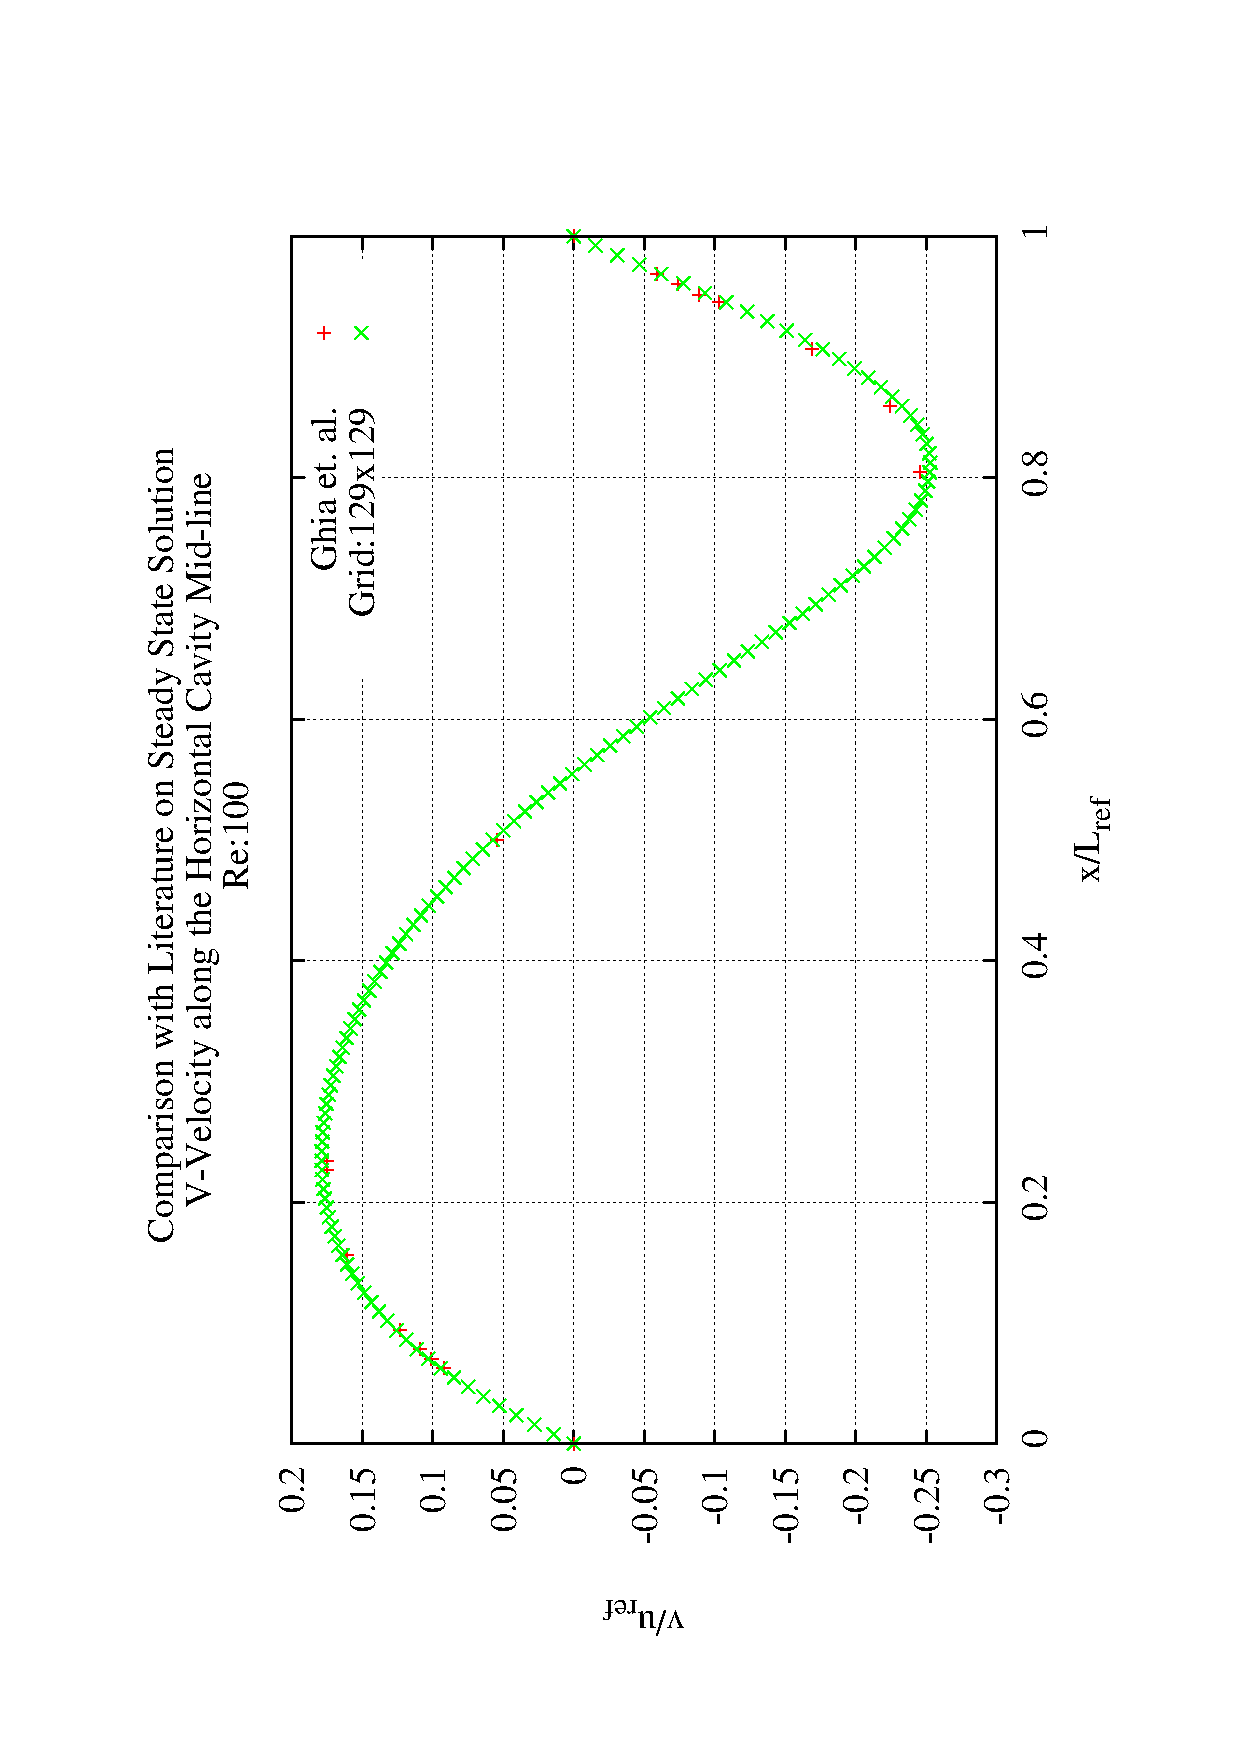
\includegraphics[width=0.9\textwidth]{plots/lit_v_100}
\caption{Steady state v-velocity as a function of x, along the horizontal cavity mid-line, at Re:100, for comparison with literature.}
\label{fig:lit_v_100}
\end{figure}


\begin{figure}[h!]
\center
\includegraphics[width=0.9\textwidth]{plots/lit_u_1000}
\caption{Steady state u-velocity as a function of y, along the vertical cavity mid-line, at Re:1000 for comparison with literature}
\label{fig:lit_u_1000}

\center
\includegraphics[width=0.9\textwidth]{plots/lit_v_1000}
\caption{Steady state v-velocity as a function of x, along the horizontal cavity mid-line, at Re:1000 for comparison with literature.}
\label{fig:lit_v_1000}
\end{figure}


	\subsection{Effect of Grid Refinement on Steady State Solution}

Having validated the fine grid solution with literature, grid spacing and its affects on the steady state solution was examined.  Simulations were run on $33x33$ and $65x65$ grids, and  were compared to simulations on the fine grid.  The u-velocity along the vertical centerline, and v-velocity along the horizontal centerline is plotted for the 3 grids in Figures \ref{fig:grs_u_100} to \ref{fig:grs_v_1000}.

\begin{figure}[h!]
\center
\includegraphics[width=0.9\textwidth]{plots/grs_u_100}
\caption{Steady state u-velocity as a function of y, along the vertical cavity mid-line, for 3 different grid sizes, at Re:100.}
\label{fig:grs_u_100}

\center
\includegraphics[width=0.9\textwidth]{plots/grs_v_100}
\caption{Steady state v-velocity as a function of x, along the horizontal cavity mid-line, for 3 different grid sizes, at Re:100.}
\label{fig:grs_v_100}
\end{figure}

\begin{figure}[h!]
\center
\includegraphics[width=0.9\textwidth]{plots/grs_u_1000}
\caption{Steady state u-velocity as a function of y, along the vertical cavity mid-line, for 3 different grid sizes, at Re:1000.}
\label{fig:grs_u_1000}

\center
\includegraphics[width=0.9\textwidth]{plots/grs_v_1000}
\caption{Steady state v-velocity as a function of x, along the vertical cavity mid-line, for 3 different grid sizes, at Re:1000.}
\label{fig:grs_v_1000}
\end{figure}

At the lower Reynolds Number, Both the medium and the coarse grid are very close to the fine grid solution.  In areas where the velocity has high curvature, the coarse grid deviates slightly off from the other two grid's velocity profile.  

For the high Reynolds Number, the medium grid deviates slightly off the fine grid solution.  The coarse grid has a significantly different profile in areas with steep gradients, near the boundaries.  The error induced by steep gradients at the boundaries propagates inwards, and as a results, the coarse grid is never really accurate.  Close to the center of the domain, where the profiles are flat, the coarse grid has a similar shape to the other grids, but error from the boundaries causes the solution to be drastically different.  Since the truncation error is proportional to $\Delta x^2$, for the numerical schemes implemented, this is not a surprising result.  The leading truncation error term is 16 times larger than that of the fine grid. As a result, truncation errors, which become significant in areas with changes in curvature, are 16 times higher in the coarse grid, then the fine grid.


